
\documentclass{article} % For LaTeX2e
\usepackage{iclr2022_conference,times}

% Optional math commands from https://github.com/goodfeli/dlbook_notation.
%%%%% NEW MATH DEFINITIONS %%%%%

\usepackage{amsmath,amsfonts,bm}

% Mark sections of captions for referring to divisions of figures
\newcommand{\figleft}{{\em (Left)}}
\newcommand{\figcenter}{{\em (Center)}}
\newcommand{\figright}{{\em (Right)}}
\newcommand{\figtop}{{\em (Top)}}
\newcommand{\figbottom}{{\em (Bottom)}}
\newcommand{\captiona}{{\em (a)}}
\newcommand{\captionb}{{\em (b)}}
\newcommand{\captionc}{{\em (c)}}
\newcommand{\captiond}{{\em (d)}}

% Highlight a newly defined term
\newcommand{\newterm}[1]{{\bf #1}}


% Figure reference, lower-case.
\def\figref#1{figure~\ref{#1}}
% Figure reference, capital. For start of sentence
\def\Figref#1{Figure~\ref{#1}}
\def\twofigref#1#2{figures \ref{#1} and \ref{#2}}
\def\quadfigref#1#2#3#4{figures \ref{#1}, \ref{#2}, \ref{#3} and \ref{#4}}
% Section reference, lower-case.
\def\secref#1{section~\ref{#1}}
% Section reference, capital.
\def\Secref#1{Section~\ref{#1}}
% Reference to two sections.
\def\twosecrefs#1#2{sections \ref{#1} and \ref{#2}}
% Reference to three sections.
\def\secrefs#1#2#3{sections \ref{#1}, \ref{#2} and \ref{#3}}
% Reference to an equation, lower-case.
\def\eqref#1{equation~\ref{#1}}
% Reference to an equation, upper case
\def\Eqref#1{Equation~\ref{#1}}
% A raw reference to an equation---avoid using if possible
\def\plaineqref#1{\ref{#1}}
% Reference to a chapter, lower-case.
\def\chapref#1{chapter~\ref{#1}}
% Reference to an equation, upper case.
\def\Chapref#1{Chapter~\ref{#1}}
% Reference to a range of chapters
\def\rangechapref#1#2{chapters\ref{#1}--\ref{#2}}
% Reference to an algorithm, lower-case.
\def\algref#1{algorithm~\ref{#1}}
% Reference to an algorithm, upper case.
\def\Algref#1{Algorithm~\ref{#1}}
\def\twoalgref#1#2{algorithms \ref{#1} and \ref{#2}}
\def\Twoalgref#1#2{Algorithms \ref{#1} and \ref{#2}}
% Reference to a part, lower case
\def\partref#1{part~\ref{#1}}
% Reference to a part, upper case
\def\Partref#1{Part~\ref{#1}}
\def\twopartref#1#2{parts \ref{#1} and \ref{#2}}

\def\ceil#1{\lceil #1 \rceil}
\def\floor#1{\lfloor #1 \rfloor}
\def\1{\bm{1}}
\newcommand{\train}{\mathcal{D}}
\newcommand{\valid}{\mathcal{D_{\mathrm{valid}}}}
\newcommand{\test}{\mathcal{D_{\mathrm{test}}}}

\def\eps{{\epsilon}}


% Random variables
\def\reta{{\textnormal{$\eta$}}}
\def\ra{{\textnormal{a}}}
\def\rb{{\textnormal{b}}}
\def\rc{{\textnormal{c}}}
\def\rd{{\textnormal{d}}}
\def\re{{\textnormal{e}}}
\def\rf{{\textnormal{f}}}
\def\rg{{\textnormal{g}}}
\def\rh{{\textnormal{h}}}
\def\ri{{\textnormal{i}}}
\def\rj{{\textnormal{j}}}
\def\rk{{\textnormal{k}}}
\def\rl{{\textnormal{l}}}
% rm is already a command, just don't name any random variables m
\def\rn{{\textnormal{n}}}
\def\ro{{\textnormal{o}}}
\def\rp{{\textnormal{p}}}
\def\rq{{\textnormal{q}}}
\def\rr{{\textnormal{r}}}
\def\rs{{\textnormal{s}}}
\def\rt{{\textnormal{t}}}
\def\ru{{\textnormal{u}}}
\def\rv{{\textnormal{v}}}
\def\rw{{\textnormal{w}}}
\def\rx{{\textnormal{x}}}
\def\ry{{\textnormal{y}}}
\def\rz{{\textnormal{z}}}

% Random vectors
\def\rvepsilon{{\mathbf{\epsilon}}}
\def\rvtheta{{\mathbf{\theta}}}
\def\rva{{\mathbf{a}}}
\def\rvb{{\mathbf{b}}}
\def\rvc{{\mathbf{c}}}
\def\rvd{{\mathbf{d}}}
\def\rve{{\mathbf{e}}}
\def\rvf{{\mathbf{f}}}
\def\rvg{{\mathbf{g}}}
\def\rvh{{\mathbf{h}}}
\def\rvu{{\mathbf{i}}}
\def\rvj{{\mathbf{j}}}
\def\rvk{{\mathbf{k}}}
\def\rvl{{\mathbf{l}}}
\def\rvm{{\mathbf{m}}}
\def\rvn{{\mathbf{n}}}
\def\rvo{{\mathbf{o}}}
\def\rvp{{\mathbf{p}}}
\def\rvq{{\mathbf{q}}}
\def\rvr{{\mathbf{r}}}
\def\rvs{{\mathbf{s}}}
\def\rvt{{\mathbf{t}}}
\def\rvu{{\mathbf{u}}}
\def\rvv{{\mathbf{v}}}
\def\rvw{{\mathbf{w}}}
\def\rvx{{\mathbf{x}}}
\def\rvy{{\mathbf{y}}}
\def\rvz{{\mathbf{z}}}

% Elements of random vectors
\def\erva{{\textnormal{a}}}
\def\ervb{{\textnormal{b}}}
\def\ervc{{\textnormal{c}}}
\def\ervd{{\textnormal{d}}}
\def\erve{{\textnormal{e}}}
\def\ervf{{\textnormal{f}}}
\def\ervg{{\textnormal{g}}}
\def\ervh{{\textnormal{h}}}
\def\ervi{{\textnormal{i}}}
\def\ervj{{\textnormal{j}}}
\def\ervk{{\textnormal{k}}}
\def\ervl{{\textnormal{l}}}
\def\ervm{{\textnormal{m}}}
\def\ervn{{\textnormal{n}}}
\def\ervo{{\textnormal{o}}}
\def\ervp{{\textnormal{p}}}
\def\ervq{{\textnormal{q}}}
\def\ervr{{\textnormal{r}}}
\def\ervs{{\textnormal{s}}}
\def\ervt{{\textnormal{t}}}
\def\ervu{{\textnormal{u}}}
\def\ervv{{\textnormal{v}}}
\def\ervw{{\textnormal{w}}}
\def\ervx{{\textnormal{x}}}
\def\ervy{{\textnormal{y}}}
\def\ervz{{\textnormal{z}}}

% Random matrices
\def\rmA{{\mathbf{A}}}
\def\rmB{{\mathbf{B}}}
\def\rmC{{\mathbf{C}}}
\def\rmD{{\mathbf{D}}}
\def\rmE{{\mathbf{E}}}
\def\rmF{{\mathbf{F}}}
\def\rmG{{\mathbf{G}}}
\def\rmH{{\mathbf{H}}}
\def\rmI{{\mathbf{I}}}
\def\rmJ{{\mathbf{J}}}
\def\rmK{{\mathbf{K}}}
\def\rmL{{\mathbf{L}}}
\def\rmM{{\mathbf{M}}}
\def\rmN{{\mathbf{N}}}
\def\rmO{{\mathbf{O}}}
\def\rmP{{\mathbf{P}}}
\def\rmQ{{\mathbf{Q}}}
\def\rmR{{\mathbf{R}}}
\def\rmS{{\mathbf{S}}}
\def\rmT{{\mathbf{T}}}
\def\rmU{{\mathbf{U}}}
\def\rmV{{\mathbf{V}}}
\def\rmW{{\mathbf{W}}}
\def\rmX{{\mathbf{X}}}
\def\rmY{{\mathbf{Y}}}
\def\rmZ{{\mathbf{Z}}}

% Elements of random matrices
\def\ermA{{\textnormal{A}}}
\def\ermB{{\textnormal{B}}}
\def\ermC{{\textnormal{C}}}
\def\ermD{{\textnormal{D}}}
\def\ermE{{\textnormal{E}}}
\def\ermF{{\textnormal{F}}}
\def\ermG{{\textnormal{G}}}
\def\ermH{{\textnormal{H}}}
\def\ermI{{\textnormal{I}}}
\def\ermJ{{\textnormal{J}}}
\def\ermK{{\textnormal{K}}}
\def\ermL{{\textnormal{L}}}
\def\ermM{{\textnormal{M}}}
\def\ermN{{\textnormal{N}}}
\def\ermO{{\textnormal{O}}}
\def\ermP{{\textnormal{P}}}
\def\ermQ{{\textnormal{Q}}}
\def\ermR{{\textnormal{R}}}
\def\ermS{{\textnormal{S}}}
\def\ermT{{\textnormal{T}}}
\def\ermU{{\textnormal{U}}}
\def\ermV{{\textnormal{V}}}
\def\ermW{{\textnormal{W}}}
\def\ermX{{\textnormal{X}}}
\def\ermY{{\textnormal{Y}}}
\def\ermZ{{\textnormal{Z}}}

% Vectors
\def\vzero{{\bm{0}}}
\def\vone{{\bm{1}}}
\def\vmu{{\bm{\mu}}}
\def\vtheta{{\bm{\theta}}}
\def\va{{\bm{a}}}
\def\vb{{\bm{b}}}
\def\vc{{\bm{c}}}
\def\vd{{\bm{d}}}
\def\ve{{\bm{e}}}
\def\vf{{\bm{f}}}
\def\vg{{\bm{g}}}
\def\vh{{\bm{h}}}
\def\vi{{\bm{i}}}
\def\vj{{\bm{j}}}
\def\vk{{\bm{k}}}
\def\vl{{\bm{l}}}
\def\vm{{\bm{m}}}
\def\vn{{\bm{n}}}
\def\vo{{\bm{o}}}
\def\vp{{\bm{p}}}
\def\vq{{\bm{q}}}
\def\vr{{\bm{r}}}
\def\vs{{\bm{s}}}
\def\vt{{\bm{t}}}
\def\vu{{\bm{u}}}
\def\vv{{\bm{v}}}
\def\vw{{\bm{w}}}
\def\vx{{\bm{x}}}
\def\vy{{\bm{y}}}
\def\vz{{\bm{z}}}

% Elements of vectors
\def\evalpha{{\alpha}}
\def\evbeta{{\beta}}
\def\evepsilon{{\epsilon}}
\def\evlambda{{\lambda}}
\def\evomega{{\omega}}
\def\evmu{{\mu}}
\def\evpsi{{\psi}}
\def\evsigma{{\sigma}}
\def\evtheta{{\theta}}
\def\eva{{a}}
\def\evb{{b}}
\def\evc{{c}}
\def\evd{{d}}
\def\eve{{e}}
\def\evf{{f}}
\def\evg{{g}}
\def\evh{{h}}
\def\evi{{i}}
\def\evj{{j}}
\def\evk{{k}}
\def\evl{{l}}
\def\evm{{m}}
\def\evn{{n}}
\def\evo{{o}}
\def\evp{{p}}
\def\evq{{q}}
\def\evr{{r}}
\def\evs{{s}}
\def\evt{{t}}
\def\evu{{u}}
\def\evv{{v}}
\def\evw{{w}}
\def\evx{{x}}
\def\evy{{y}}
\def\evz{{z}}

% Matrix
\def\mA{{\bm{A}}}
\def\mB{{\bm{B}}}
\def\mC{{\bm{C}}}
\def\mD{{\bm{D}}}
\def\mE{{\bm{E}}}
\def\mF{{\bm{F}}}
\def\mG{{\bm{G}}}
\def\mH{{\bm{H}}}
\def\mI{{\bm{I}}}
\def\mJ{{\bm{J}}}
\def\mK{{\bm{K}}}
\def\mL{{\bm{L}}}
\def\mM{{\bm{M}}}
\def\mN{{\bm{N}}}
\def\mO{{\bm{O}}}
\def\mP{{\bm{P}}}
\def\mQ{{\bm{Q}}}
\def\mR{{\bm{R}}}
\def\mS{{\bm{S}}}
\def\mT{{\bm{T}}}
\def\mU{{\bm{U}}}
\def\mV{{\bm{V}}}
\def\mW{{\bm{W}}}
\def\mX{{\bm{X}}}
\def\mY{{\bm{Y}}}
\def\mZ{{\bm{Z}}}
\def\mBeta{{\bm{\beta}}}
\def\mPhi{{\bm{\Phi}}}
\def\mLambda{{\bm{\Lambda}}}
\def\mSigma{{\bm{\Sigma}}}

% Tensor
\DeclareMathAlphabet{\mathsfit}{\encodingdefault}{\sfdefault}{m}{sl}
\SetMathAlphabet{\mathsfit}{bold}{\encodingdefault}{\sfdefault}{bx}{n}
\newcommand{\tens}[1]{\bm{\mathsfit{#1}}}
\def\tA{{\tens{A}}}
\def\tB{{\tens{B}}}
\def\tC{{\tens{C}}}
\def\tD{{\tens{D}}}
\def\tE{{\tens{E}}}
\def\tF{{\tens{F}}}
\def\tG{{\tens{G}}}
\def\tH{{\tens{H}}}
\def\tI{{\tens{I}}}
\def\tJ{{\tens{J}}}
\def\tK{{\tens{K}}}
\def\tL{{\tens{L}}}
\def\tM{{\tens{M}}}
\def\tN{{\tens{N}}}
\def\tO{{\tens{O}}}
\def\tP{{\tens{P}}}
\def\tQ{{\tens{Q}}}
\def\tR{{\tens{R}}}
\def\tS{{\tens{S}}}
\def\tT{{\tens{T}}}
\def\tU{{\tens{U}}}
\def\tV{{\tens{V}}}
\def\tW{{\tens{W}}}
\def\tX{{\tens{X}}}
\def\tY{{\tens{Y}}}
\def\tZ{{\tens{Z}}}


% Graph
\def\gA{{\mathcal{A}}}
\def\gB{{\mathcal{B}}}
\def\gC{{\mathcal{C}}}
\def\gD{{\mathcal{D}}}
\def\gE{{\mathcal{E}}}
\def\gF{{\mathcal{F}}}
\def\gG{{\mathcal{G}}}
\def\gH{{\mathcal{H}}}
\def\gI{{\mathcal{I}}}
\def\gJ{{\mathcal{J}}}
\def\gK{{\mathcal{K}}}
\def\gL{{\mathcal{L}}}
\def\gM{{\mathcal{M}}}
\def\gN{{\mathcal{N}}}
\def\gO{{\mathcal{O}}}
\def\gP{{\mathcal{P}}}
\def\gQ{{\mathcal{Q}}}
\def\gR{{\mathcal{R}}}
\def\gS{{\mathcal{S}}}
\def\gT{{\mathcal{T}}}
\def\gU{{\mathcal{U}}}
\def\gV{{\mathcal{V}}}
\def\gW{{\mathcal{W}}}
\def\gX{{\mathcal{X}}}
\def\gY{{\mathcal{Y}}}
\def\gZ{{\mathcal{Z}}}

% Sets
\def\sA{{\mathbb{A}}}
\def\sB{{\mathbb{B}}}
\def\sC{{\mathbb{C}}}
\def\sD{{\mathbb{D}}}
% Don't use a set called E, because this would be the same as our symbol
% for expectation.
\def\sF{{\mathbb{F}}}
\def\sG{{\mathbb{G}}}
\def\sH{{\mathbb{H}}}
\def\sI{{\mathbb{I}}}
\def\sJ{{\mathbb{J}}}
\def\sK{{\mathbb{K}}}
\def\sL{{\mathbb{L}}}
\def\sM{{\mathbb{M}}}
\def\sN{{\mathbb{N}}}
\def\sO{{\mathbb{O}}}
\def\sP{{\mathbb{P}}}
\def\sQ{{\mathbb{Q}}}
\def\sR{{\mathbb{R}}}
\def\sS{{\mathbb{S}}}
\def\sT{{\mathbb{T}}}
\def\sU{{\mathbb{U}}}
\def\sV{{\mathbb{V}}}
\def\sW{{\mathbb{W}}}
\def\sX{{\mathbb{X}}}
\def\sY{{\mathbb{Y}}}
\def\sZ{{\mathbb{Z}}}

% Entries of a matrix
\def\emLambda{{\Lambda}}
\def\emA{{A}}
\def\emB{{B}}
\def\emC{{C}}
\def\emD{{D}}
\def\emE{{E}}
\def\emF{{F}}
\def\emG{{G}}
\def\emH{{H}}
\def\emI{{I}}
\def\emJ{{J}}
\def\emK{{K}}
\def\emL{{L}}
\def\emM{{M}}
\def\emN{{N}}
\def\emO{{O}}
\def\emP{{P}}
\def\emQ{{Q}}
\def\emR{{R}}
\def\emS{{S}}
\def\emT{{T}}
\def\emU{{U}}
\def\emV{{V}}
\def\emW{{W}}
\def\emX{{X}}
\def\emY{{Y}}
\def\emZ{{Z}}
\def\emSigma{{\Sigma}}

% entries of a tensor
% Same font as tensor, without \bm wrapper
\newcommand{\etens}[1]{\mathsfit{#1}}
\def\etLambda{{\etens{\Lambda}}}
\def\etA{{\etens{A}}}
\def\etB{{\etens{B}}}
\def\etC{{\etens{C}}}
\def\etD{{\etens{D}}}
\def\etE{{\etens{E}}}
\def\etF{{\etens{F}}}
\def\etG{{\etens{G}}}
\def\etH{{\etens{H}}}
\def\etI{{\etens{I}}}
\def\etJ{{\etens{J}}}
\def\etK{{\etens{K}}}
\def\etL{{\etens{L}}}
\def\etM{{\etens{M}}}
\def\etN{{\etens{N}}}
\def\etO{{\etens{O}}}
\def\etP{{\etens{P}}}
\def\etQ{{\etens{Q}}}
\def\etR{{\etens{R}}}
\def\etS{{\etens{S}}}
\def\etT{{\etens{T}}}
\def\etU{{\etens{U}}}
\def\etV{{\etens{V}}}
\def\etW{{\etens{W}}}
\def\etX{{\etens{X}}}
\def\etY{{\etens{Y}}}
\def\etZ{{\etens{Z}}}

% The true underlying data generating distribution
\newcommand{\pdata}{p_{\rm{data}}}
% The empirical distribution defined by the training set
\newcommand{\ptrain}{\hat{p}_{\rm{data}}}
\newcommand{\Ptrain}{\hat{P}_{\rm{data}}}
% The model distribution
\newcommand{\pmodel}{p_{\rm{model}}}
\newcommand{\Pmodel}{P_{\rm{model}}}
\newcommand{\ptildemodel}{\tilde{p}_{\rm{model}}}
% Stochastic autoencoder distributions
\newcommand{\pencode}{p_{\rm{encoder}}}
\newcommand{\pdecode}{p_{\rm{decoder}}}
\newcommand{\precons}{p_{\rm{reconstruct}}}

\newcommand{\laplace}{\mathrm{Laplace}} % Laplace distribution

\newcommand{\E}{\mathbb{E}}
\newcommand{\Ls}{\mathcal{L}}
\newcommand{\R}{\mathbb{R}}
\newcommand{\emp}{\tilde{p}}
\newcommand{\lr}{\alpha}
\newcommand{\reg}{\lambda}
\newcommand{\rect}{\mathrm{rectifier}}
\newcommand{\softmax}{\mathrm{softmax}}
\newcommand{\sigmoid}{\sigma}
\newcommand{\softplus}{\zeta}
\newcommand{\KL}{D_{\mathrm{KL}}}
\newcommand{\Var}{\mathrm{Var}}
\newcommand{\standarderror}{\mathrm{SE}}
\newcommand{\Cov}{\mathrm{Cov}}
% Wolfram Mathworld says $L^2$ is for function spaces and $\ell^2$ is for vectors
% But then they seem to use $L^2$ for vectors throughout the site, and so does
% wikipedia.
\newcommand{\normlzero}{L^0}
\newcommand{\normlone}{L^1}
\newcommand{\normltwo}{L^2}
\newcommand{\normlp}{L^p}
\newcommand{\normmax}{L^\infty}

\newcommand{\parents}{Pa} % See usage in notation.tex. Chosen to match Daphne's book.

\DeclareMathOperator*{\argmax}{arg\,max}
\DeclareMathOperator*{\argmin}{arg\,min}

\DeclareMathOperator{\sign}{sign}
\DeclareMathOperator{\Tr}{Tr}
\let\ab\allowbreak


\usepackage{url}
\usepackage{hyperref}
% \usepackage{subfig}
\usepackage{graphicx}
\usepackage{cleveref}
% \usepackage[disable]{todonotes}
\usepackage{todonotes}
\setuptodonotes{inline}
\usepackage{tikz}
\usepackage{caption}
\usepackage{subcaption}
\usepackage{gensymb}

\definecolor{blue1}{RGB}{0,102,189}
\definecolor{blue2}{RGB}{98,160,214}
\definecolor{my_orange}{RGB}{243,98,33}
\definecolor{mygreen}{RGB}{30,106,57}
\definecolor{mypurple}{RGB}{91,39,125}
\definecolor{myred}{RGB}{241,13,12}

\def\boxit#1{%
  \smash{\color{black}\fboxrule=1pt\relax\fboxsep=2pt\relax%
  \llap{\rlap{\fbox{\vphantom{0}\makebox[#1]{}}}~}}\ignorespaces
}
% library

\colorlet{incolor}{tumorange}
\colorlet{outcolor}{tumblue}

\usepackage{tikz-dimline}

\tikzset{inNode/.style={draw=incolor, fill=incolor, circle, inner sep=1.5pt}}
\tikzset{outNode/.style={draw=outcolor,  fill=outcolor, circle, inner sep=1pt}}
\tikzset{projNode/.style={draw=outcolor, fill=outcolor, circle, inner sep=1pt}}

\usetikzlibrary{shapes.arrows, fadings, calc, positioning}
\tikzfading[name=fade right,
  left color=transparent!0, right color=transparent!100]
\tikzfading[name=fade left,
  left color=transparent!100, right color=transparent!0]
\tikzfading[name=fade top,
  bottom color=transparent!0, top color=transparent!100]
  
\pgfdeclarelayer{bg}    % declare background layer
\pgfdeclarelayer{fg}    % declare foreground layer
\pgfsetlayers{bg,main,fg}  % set the order of the layers (main is the standard layer)

\definecolor{participantAcolor}{RGB}{243,98,33}
\definecolor{participantBcolor}{RGB}{0,102,189}
%\definecolor{participantCcolor}{RGB}{253,215,130}
\definecolor{participantCcolor}{RGB}{66,70,50}
\definecolor{cplColor}{RGB}{0,0,0}
\definecolor{preciceColor}{RGB}{ 161, 177, 25}

%%% CI colors, https://portal.mytum.de/corporatedesign/regeln/index_styleguide p.20

\definecolor{ci_pantone300}{RGB}{ 0, 101, 189}

\definecolor{ci_pantone301}{RGB}{ 0, 82, 147}
\definecolor{ci_pantone540}{RGB}{ 0, 51, 89}

\definecolor{ci_pantone283}{RGB}{ 152, 198, 234}
\definecolor{ci_pantone542}{RGB}{ 100, 160, 200}
\definecolor{ci_ivory}{RGB}{ 218, 215, 203}
\definecolor{ci_orange}{RGB}{ 227, 114, 34}
\definecolor{ci_green}{RGB}{ 162, 173, 0}  



%\title{Formatting Instructions for ICLR 2022 \\ Conference Submissions}
\title{Surrogate Modelling of Thermal Plumes for Shallow Subsurface Temperature Approximation}

% Authors must not appear in the submitted version. They should be hidden
% as long as the \iclrfinalcopy macro remains commented out below.
% Non-anonymous submissions will be rejected without review.

\author{Antiquus S.~Hippocampus, Natalia Cerebro \& Amelie P. Amygdale \thanks{ Use footnote for providing further information
about author (webpage, alternative address)---\emph{not} for acknowledging
funding agencies.  Funding acknowledgements go at the end of the paper.} \\
Department of Computer Science\\
Cranberry-Lemon University\\
Pittsburgh, PA 15213, USA \\
\texttt{\{hippo,brain,jen\}@cs.cranberry-lemon.edu} \\
\And
Ji Q. Ren \& Yevgeny LeNet \\
Department of Computational Neuroscience \\
University of the Witwatersrand \\
Joburg, South Africa \\
\texttt{\{robot,net\}@wits.ac.za} \\
\AND
Coauthor \\
Affiliation \\
Address \\
\texttt{email}
}

% The \author macro works with any number of authors. There are two commands
% used to separate the names and addresses of multiple authors: \And and \AND.
%
% Using \And between authors leaves it to \LaTeX{} to determine where to break
% the lines. Using \AND forces a linebreak at that point. So, if \LaTeX{}
% puts 3 of 4 authors names on the first line, and the last on the second
% line, try using \AND instead of \And before the third author name.

\newcommand{\fix}{\marginpar{FIX}}
\newcommand{\new}{\marginpar{NEW}}

%\iclrfinalcopy % Uncomment for camera-ready version, but NOT for submission.
\begin{document}


\maketitle

\begin{abstract}
   Climate control of buildings makes up a significant portion of global energy consumption, with groundwater heat pumps providing a suitable alternative.
   %With the climate crisis worsening extreme weather events and the slow change towards renewable energies, the desire for better energy efficiency results in a lot of new developments considering groundwater heat pumps.
   To prevent possibly negative interactions between heat pumps throughout a city, city planners have to optimize their layouts in the future.
   We develop a novel data-driven approach for building small-scale surrogates for modelling the thermal plumes generated by groundwater heat pumps in the surrounding subsurface water.
   Building on a data set generated from numerical simulations, we train a convolutional neural network for predicting steady-state subsurface temperature fields from a given subsurface velocity field.
   We show that compared to existing models ours can capture more complex dynamics while still being quick to compute and achieving a reasonable error rate.
\end{abstract}

\section{Introduction}
\label{sec:intro}

Heating and cooling of buildings has garnered attention in recent years, especially as the world moves towards renewable sources of energy. 
%It is estimated up to three quarters of the worlds fossil fuels used in buildings goes towards heating (The Economist).
%In a world moving towards renewables ernergy as main 
One focus recently has been on using shallow geothermal energy through groundwater heat pumps (GWHP) \citep{Halilovic2022}. 
As the groundwater temperature is relatively stable year round, GWHPs are able to use this source to both heat and cool buildings. %(https://www.energy.gov/energysaver/geothermal-heat-pumps) 
As cities move towards installing more GWHPs, assessing and optimizing their influence on the subsurface is required. 
Installing GWHPs without any restrictions could result in situations where negative interaction occurs \citep{Garcia2020, Daemi2019}. 
GWHPs operate by extracting water from an extraction well, either heating or cooling this fluid, and re-injecting it back into the subsurface.  
The local temperature changes around the injection well, and a thermal plume develops due to the diffusion and advection of this water in the subsurface. 
This thermal plume can propagate downstream and interact with other GWHPs or even recirculate into its own extraction well, causing interference. 
This requires careful planning of the layout and operational loads of GWHPs \citep{Beck2013}. 
To provide an accurate assessment of the groundwater temperatures due to the usage of many heat pumps, high-fidelity subsurface flow simulations are required \citep{Meng2019}. 
Furthermore, to optimize the layout and usage of a large number of GWHPs on this scale requires many high-fidelity simulation runs, making large optimization scenarios infeasible.

A common solution is to use surrogate models, also known as low-fidelity models, which are computationally cheap to solve the optimization problem \citep{Sbai2019, Nagoor2019, Robinson2012}. 
To help optimize the layout of potentially thousands of GWHPs, surrogate models could be used to determine the local temperature influence that each GWHP has on the groundwater temperature. 
As the thermal influence of one heat pump can be computed fast and cheaply, many such evaluations can be performed to determine the influence of multiple heat pumps in a system. 
This can be used to provide either a semi-optimised solution, or to evaluate the influence of one heat pump on other previously installed heat pumps. 

%We need to model the local temperature variation that develops, i.e. determine the thermal plume. 
Analytical solutions provide a computationally cheap solution to predict the thermal plume \citep{Pophillat2020}, but suffer from several disadvantages. 
They often do not account for variations in the groundwater parameters in space, such as varying permeability field, pressure gradients and velocity fields. 
This results in the thermal plume extending in one direction only for the analytical solutions ( Fig.~\ref{analyticalPlume}), however, the thermal plumes may actually change their direction due to heterogeneous groundwater parameters or obstructions. 

In a typical application the optimization problem would consist of an area with many GWHP's (such as in Fig.~\ref{large_example}, and potentially much larger areas), with known geological parameters; Spatially varying permeability field and pressure boundary conditions. 
The surrogate model must be able to provide the local temperature variation (thermal plume) around each individual GWHP (Fig.~\ref{fig:sub1_temp}), and we can determine which GWHPs might interact with each other.

\begin{figure}[!htb]
\centering
\begin{subfigure}{.5\textwidth}
  \centering
  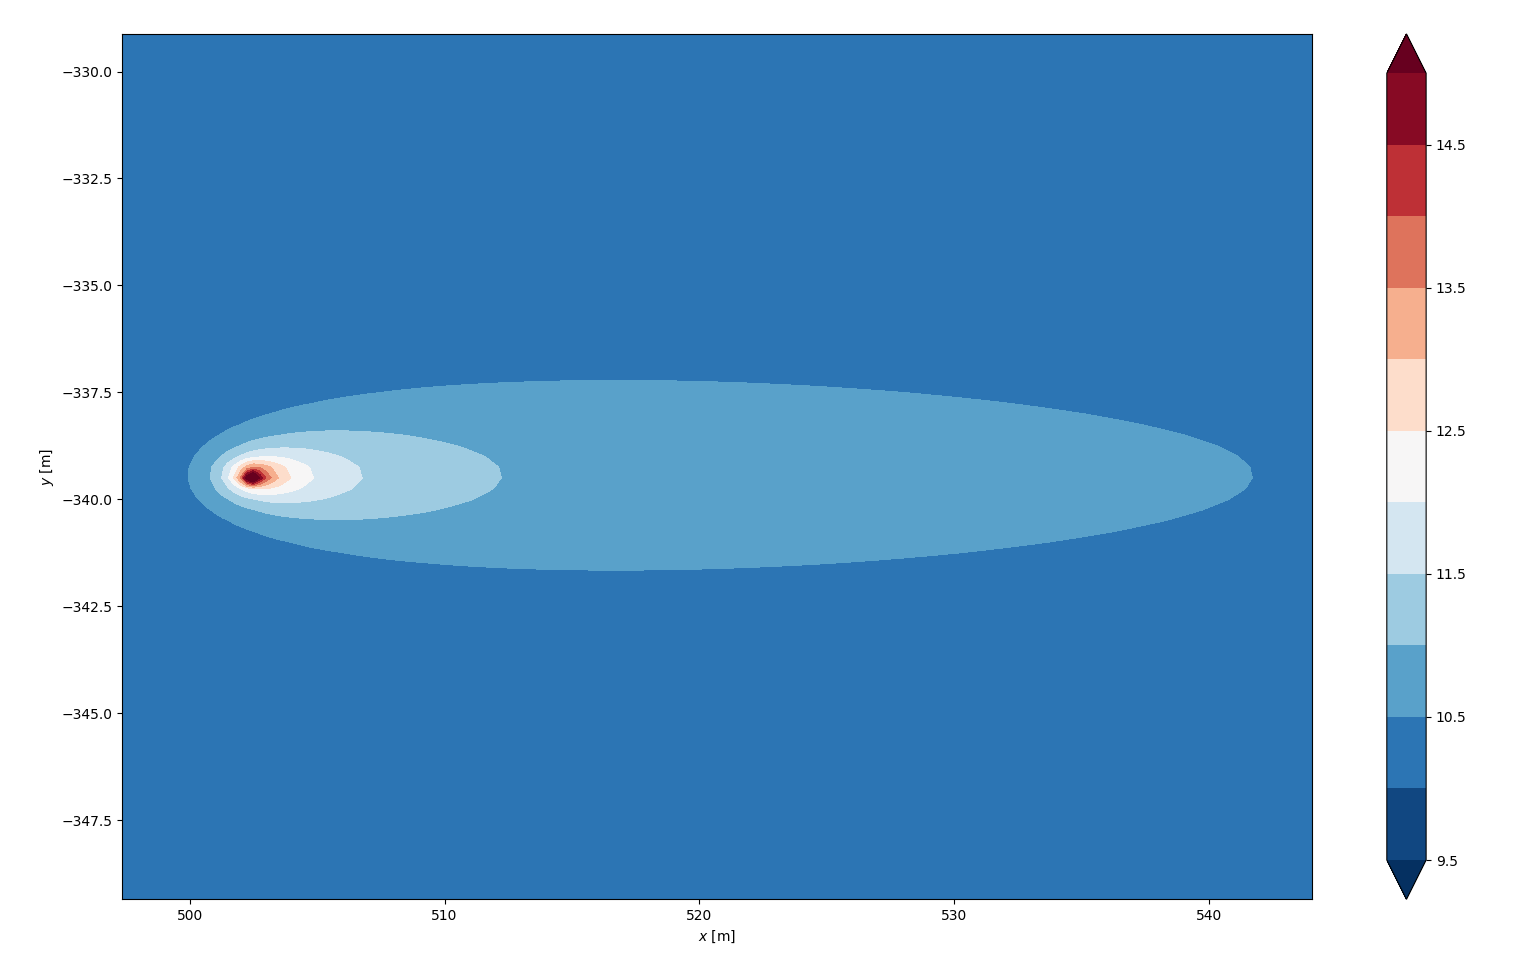
\includegraphics[width=.8\linewidth]{analyticalPlume.png}
  \caption{Analytical thermal plume}
  \label{analyticalPlume}
\end{subfigure}%
\begin{subfigure}{.5\textwidth}
  \centering
  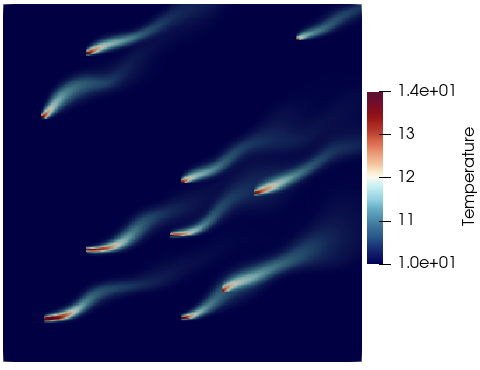
\includegraphics[width=.8\linewidth]{large_temp_example_2.png}
  \caption{Temperature field with 10 GWHPs scattered throughout the domain.}
  \label{large_example}
\end{subfigure}
\caption{The thermal plume developed by (a) GWHP derived from the LAHM model \citep{Pophillat2020} and (b) 10 GWHPs in a large domain using a spatially varying permeability field. The thermal plume in (a) is uni-directional for the analytical model, and is dependent only on the parameters at the location of reinjection. A more realistic example in (b) shows that the thermal plumes follow the velocity direction of the subsurface.}
\label{fig:plume_and_overview}
\end{figure}

%One crucial development of the past decade to achieve this is the widespread adoptioln of more energy efficient and carbon-free techniques for heating and cooling urban buildings.
%A central role plays the usage of heat pumps extracting energy from subsurface groundwater 

%Establishing this technology on a large city-wide scale however, requires some regulatory oversight for the locations and energetic dimensions of installed heat pumps.
%Installing these without any restrictions might result in situations where the heat injection/substraction from one pump might negatively impact the performance of another pump down-stream.

%In a first step to address this optimization problem this work aims at providing a web-based tool for city planners to quickly test out different placement scenarios.
%Using a machine learning surrogates we want to predict physically accurate temperature fields in real-time based in the users input and measured groundwater flow fields of a large European city.

%- general motivation (large scale heat pump adoption requires optimization of placements etc.)
%\begin{enumerate}
%\item The large scale roll-out of shallow groundwater heat pumps often results in thermal interference of the installed heat pumps.
%\item This requires optimization of placement and usage of heat pumps to manage the subsurface thermal resource.
%\item Current analytical formulas are too simplistic.
%\end{enumerate}

%- geokw project outline (possibly de-anonymizing?) \\
%KD: We can remove GeoKW and I can explain the project. The web-app isnt live so they wouldn't be able to find it.

%- specific application in web-based real-time context -> requires fast online evaluation
%\begin{enumerate}
%\item Specific application is the optimization, as this is crazy expensive. Try to reduce computational time of the optimization.
%\item Second application is a web-based planning tool, which gives energy planners an easy tool to assess compatability.
%\end{enumerate}


\subsection*{Related Work}
\todo[disable]{extend, less PINN focus}
The usage of machine learning based surrogates for physical applications has increased dramatically in recent years \citep{Vinuesa2021,Chen2021,Zhu2019}.
There have been purely supervised learning approaches put forth \citep{nn_pde_data} with multiple variations using e.g. convolutional neural networks (CNNs) \citep{nn_pde_cnn, Thuerey2019} or LSTMs \citep{dl_lstm} for temporal modelling.
%Equally the number of different approaches is quite diverse.
Another promising line of research are physics-informed neural networks (PINNs), where a neural network is trained to satisfy some specific boundary-value problem \citep{pinn,pinn_subsurface,pinn_hfm,pinn_pathologies,Gao2021}. 
Given a partial differential equation (PDE), the residual is added to the networks loss function which is then trained to minimize this residual.
% Therefore, the PINN output should satisfy the underlying physical laws of the PDE. 
% Other works utilise PINN's to provide error correction for coarse scale models \citep{Gao2021}. 
%One of these are physics-informed methods where a neural network (NN) is trained to approximate the solution of a specific boundary-value problem \citep{pinn}.
%This works by adding the PDE residual of the underlying equations to the loss function and thus optimizing the network for solutions which obey the underlying physical laws.
Other works follow a coupled approach such as CFDNet \citep{cfdnet} where a neural network surrogate is used as a pre-conditioner inside a traditional numerical solver or e.g \citet{BECK2019108910} where a neural network is used to model closure terms for turbulent flows.
In this work, we focus on a purely supervised CNN approach for making new predictions by focusing on a very confined flow domain.


\section{Method}
\label{sec:method}

% In this section we describe the model setup and data generation. 

% \subsection*{Surrogate Model}

The surrogate model only needs to solve for the local temperature field around a GWHP. 
% We solve for the boundary value problem using a finite volume subsurface solver to determine the pressure field, velocity field and temperature field. 
%However, we assume that the velocity field is is only locally influenced by a GWHP, and we can therefore run our model without any GWHPs installed to determine an initial pressure and velocity field.  
We assume that the subsurface temperature is domniated by the advection term in the darcy flow equations (Eq.~\ref{eq:energy}), and the temperature profile follows the velocity field profile. 
Therefore, our aim is to develop a surrogate model that uses the spatially varying, steady-state groundwater velocity field as an input, and outputs the thermal plume that develops due to the additional of a single GWHP in a smaller domain. 


\subsection*{Data Generation}

% \todo{- Data description}
% - Data generation (using PFLOTRAN)
% \begin{enumerate}
% \item Randomly generate permeability fields and pressure boundaries to generate velocity fields.
% \item Simulate this with added heat flux to determine temperatures
% \end{enumerate}

In order to train the neural network, we need to provide enough training data such that the thermal plume can be accurately captured. We use PFLOTRAN \citep{pflotran-paper} to perform high-fidelity subsurface simulations.
We solve for the boundary value problem using a finite volume subsurface solver to determine the pressure field, velocity field and temperature field.
We consider a 2D domain with directions $x$ and $y$, and darcy velocities $\vq = (q_x, q_y)$.
% The darcy velocities are used as inputs to the neural network.
The training data simulations are performed on a 64x64 structured grid with 4096 cells, covering an area of 128$m$ $\times$ 128$m$ $\times$ 1$m$. The GWHP is modelled by injecting fluid of 0.05 $kg \cdot s^{-1}$ at 15 \degree C at the center of the domain, and run for a total of 720 days to achieve a pseudo steady-state solution. The domain temperature is set to 10 \degree C at time T $=$ 0.



%\begin{figure}[h]
%\centering
%\begin{tikzpicture}[scale=2, every node/.style={font=\small}]

%\coordinate(origin) at (0,0);

%\coordinate(fluidWidth) at (2,0);
%\coordinate(fluidHeight) at (0,2);

%\coordinate(fluidBottomLeft) at ($(origin)$);
%\coordinate(fluidTopRight) at ($(origin) + (fluidWidth) + (fluidHeight)$);

%\draw[fill=participantBcolor!50](fluidBottomLeft) rectangle (fluidTopRight);
%\dimline[extension start length=0, extension end length=0] {($(0,2)+(0,.21)$)}{($(2,2)+(0,.21)$)}{$L$};

%\draw($(0.05,0.98)$) -- node[right, black, align=right]{$\Gamma_\text{inlet}$} ($(0.05,0.98)$);  % inlet
%\draw($(0.85,0.15)$) -- node[right, black, align=right]{$\Gamma_\text{inlet}$} ($(0.85,0.15)$);  % inlet
%\draw($(1.5,0.98)$) -- node[right, black, align=right]{$\Gamma_\text{outlet}$} ($(1.5,0.98)$);  % outlet
%\draw($(0.855,1.78)$) -- node[right, black, align=right]{$\Gamma_\text{outlet}$} ($(0.85,1.78)$);  % outlet

%\end{tikzpicture}
%\end{figure}

\begin{figure}[!htb]
\centering
\begin{subfigure}{.33\textwidth}
  \centering
  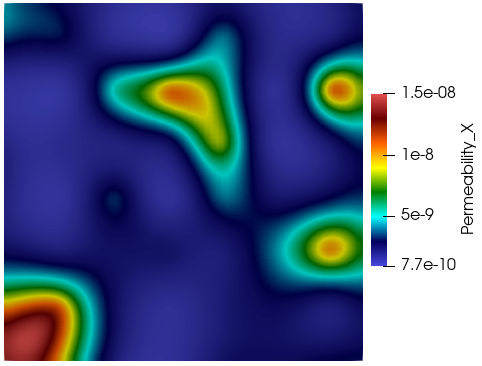
\includegraphics[width=.8\linewidth]{perm_example.png}
  \caption{Permeability Field}
  \label{fig:sub1_perm}
\end{subfigure}%
\begin{subfigure}{.33\textwidth}
  \centering
  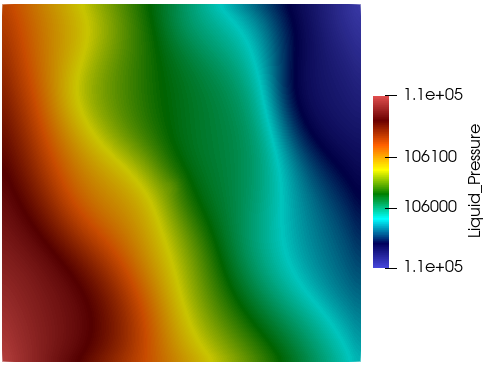
\includegraphics[width=.8\linewidth]{pressure_example.png}
  \caption{Pressure Field}
  \label{fig:sub1_pressure}
\end{subfigure}
\begin{subfigure}{.33\textwidth}
  \centering
  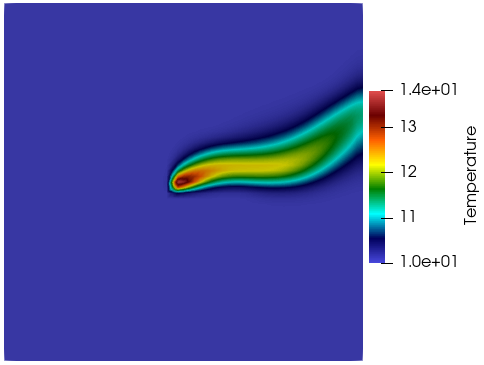
\includegraphics[width=.8\linewidth]{temp_example.png}
  \caption{Temperature Field}
  \label{fig:sub1_temp}
\end{subfigure}%
\caption{The permeability field (a), pressure field (b) and temperature field (c) for a training data example. The temperature plume that develops from the GWHP is not uni-directional like the analytical solutions, and depends on the velocity magnitude and direction.}
\label{fig:data_example}
\end{figure}


%\todo{to train fast surrogate we need data}

%\todo{data is generated using FV solver pflotran for different configurations}

The training data is generated by varying the permeability field and pressure boundary conditions to generate randomly varying velocity fields.
The permeability field is generated by randomly assigning values between $4.1 \cdot 10^{-8}$ and $2.1 \cdot 10^{-9}$ at various points on a $4 \times 4$, $6 \times 6$ and $8 \times 8$ square grid throughout the domain. We use the Python library \textit{Random} to pseudo-randomly generate the permeability values. These values are then mapped to the PFLOTRAN grid using that radial basis function (RBF) interpolation method with global thin-plate-splines basis functions.
%These values are then rescaled and converted into the permeability field values.
An example permeability field in shown in Fig.~\ref{fig:sub1_perm}.
%We created 6 sets of data with which to train the model.
%Three data sets use a relatively coarse $4 \times 4$ grid for the RBF interpolation onto the PFLOTRAN grid, and another three data sets with a $8 \times 8$ grid. 
%Each of these three data sets have a maximum and minimum permeability value of: $1.1 \cdot 10^{-7}$ - $5.6 \cdot 10^{-9}$, $4.1 \cdot 10^{-8}$ - $2.1 \cdot 10^{-9}$ and $1.5 \cdot 10^{-8}$ - $7.6 \cdot 10^{-10}$.
The pressure gradient applied to the domain is galso enerated using the \textit{random} library in Python. Two random values for the $x$ and $y$ direction of the gradient are applied. The pressure values are 
% Only positive gradient values are applied in the $x$ direction $(0 , 1)$, whereas the $y$ direction is allowed to vary between $(-1 , 1)$.
% This generates velocity fields in the positive $x$ direction only, however we can rotate the data during training. 
This allows us to generate many varying velocity fields, and due to the small size of the FV solver, the simulations to calculate a stead-state temperature field $T$ are computationally feasible.
For more details regarding the simulation setup see Appendix \ref{ap:sim_details}.

\todo[disable]{underlying equations are the (stationary) Richards flow equations}
\todo[disable]{generate arbitrary configurations with smooth random flow fields}
\todo[disable]{injection in the middle of the domain leads to some temperature plume}
\todo[disable]{we solve a bunch of these until a quasi-stationary state is achieved}

\subsection*{Preprocessing}
Before using the data we apply some preprocessing to aid the training process.
First, we substract $10 \degree C$ from all temperature values as this is the initial groundwater temperature we set for our simulation.
Then, we normalize each quantity (darcy flow $(q_x, q_y)$ and temperature $T$) separately by centering and scaling the data such that they are restricted to the $[-1, 1]$ range.
%\todo{temperature is always offset by 10, what was the reason for that again?}
This often simplifies the learning task for NNs as has been shown previously e.g. in \citep{LeCun2012,Wiesler2011}.
Additionally, we augment and extend the data set by appending randomly rotated input and target images resulting in a larger data set for more robust results.


\subsection*{Model}
\todo[disable]{as surrogate we use a TurbNet structure}
\begin{figure}[!htb]
   \centering
   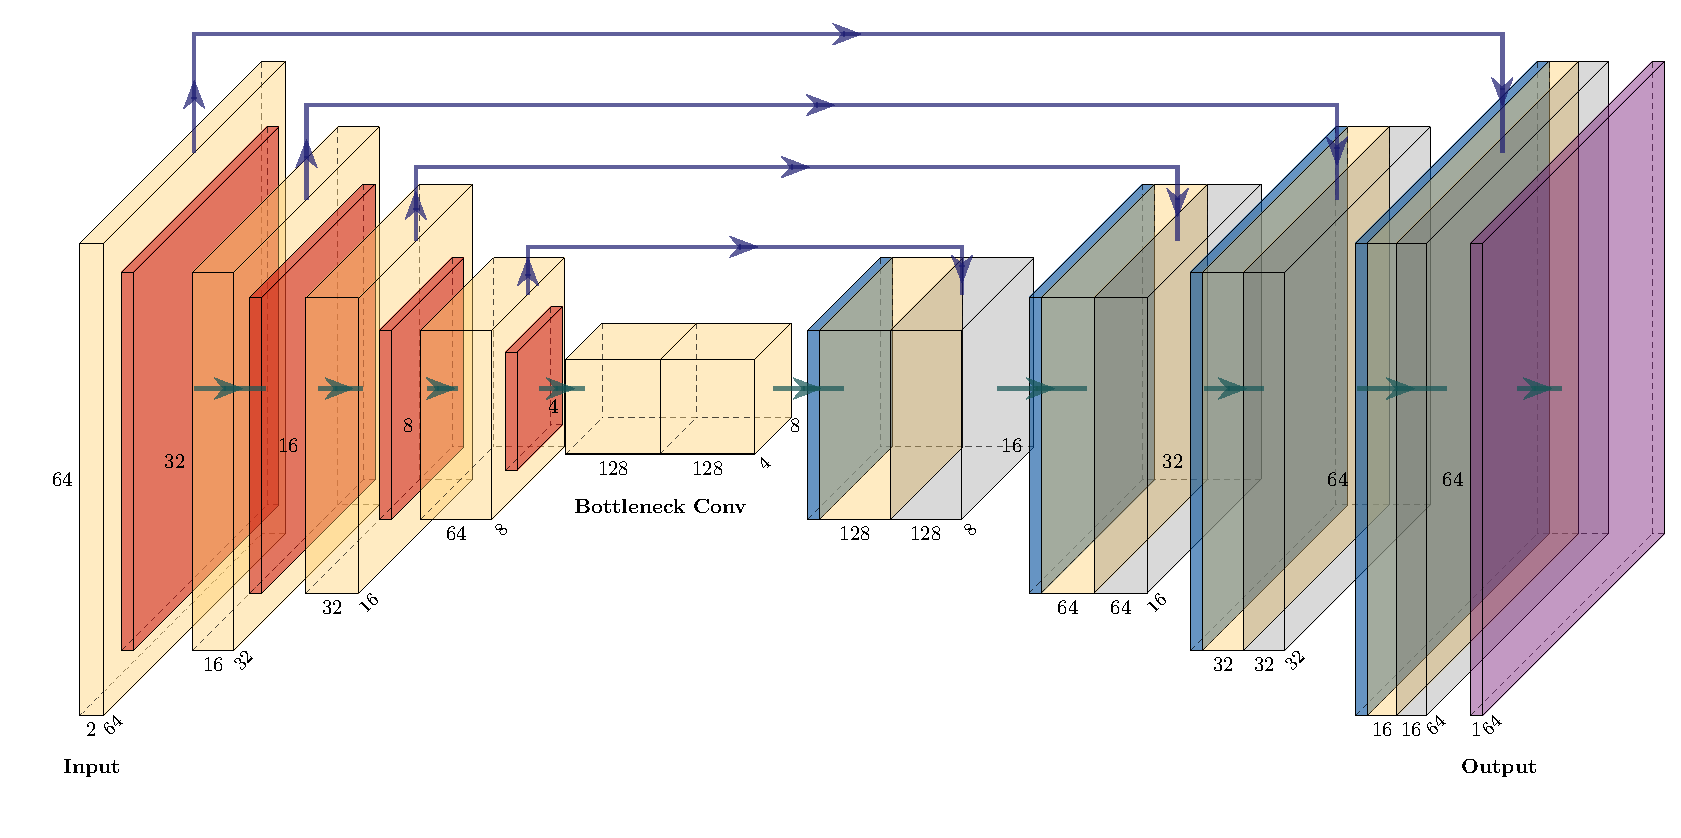
\includegraphics[width=0.8\textwidth]{img/arch.pdf}
   \caption{Visualization of the U-net type network architecture. The encoder and decoder paths feature 2D convolutions and ReLU activation functions. Both paths are connected via skip connections in each level.}
   \label{fig:arch}
\end{figure}

For the surrogate model, we choose a slightly modified version of the ``TurbNet'' architecture as described in \citet{Thuerey2019} which in turn can be considered a variant of the ``U-net'' \citep{Ronneberger2015}.
The input is given as a two-channel image with $64\times64$ pixel values corresponding the the darcy flow $\vq$.
The general shape is similar to a simple ``U-net'' where the input is convolved into coarser and coarser features on a contracting path until a bottleneck level is reached. 
%This is done until a bottleneck level is reached. 
From this on the feature channels are again de-convolved in a symmetric fashion upwards.
Additionally, each step in the hierarchy also includes a skip connection, copying intermediate results from the contracting path and concatenating it feature wise to the results of the expanding path.
As an output, the network produces a single channel image at the same $64\times64$ resolution of the predicted temperature field.
A graphical overview of the architecture is depicted in Fig.~\ref{fig:arch}.
In contrast to \citep{Thuerey2019} we raised the feature size of the bottleneck path.
Our assumption is that features which are convolved down to a single pixel value don't hold much relevant information anymore and we can thus save some model complexity.
Additionally, we lowered the amount of channels in each block as our experiments showed good results even with fewer parameters.
This approach allows us to directly predict a stationary temperature plume for any given flow field.


\todo[disable]{why did we choose this?}
\todo[disable]{- allows us to directly predict stationary temperature plume for a given flow field}
\todo[disable]{- can then be used in a real-time setting to make predictions for the website user}

\section{Results}
\label{sec:results}

% \begin{figure}[htb]
%    \centering
%    \includegraphics[width=5cm]{example-image-a}
%    \caption{Example visualization of a single data sample. Streamlines represent the darcy flow velocity overlay over a plot of the temperature.}
% \end{figure}

\begin{figure}[!htb]
   \centering
   \begin{subfigure}{0.9\textwidth}
      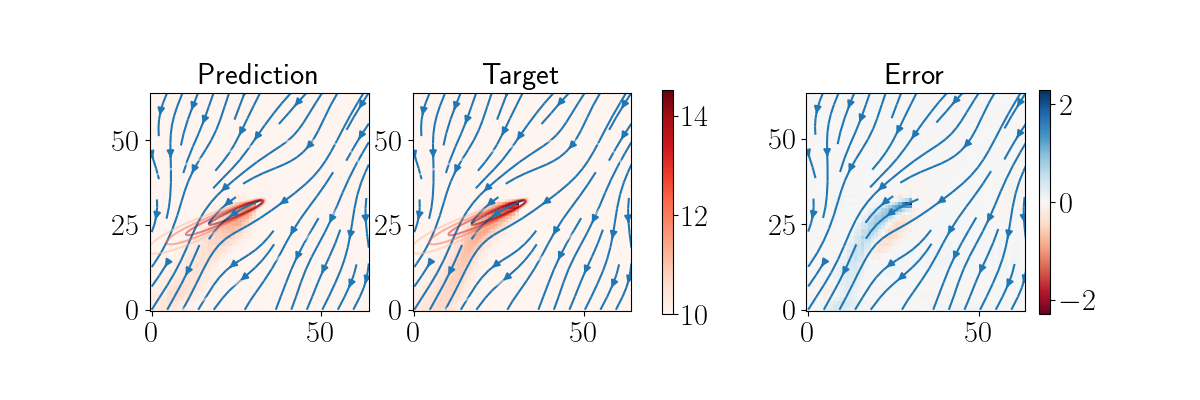
\includegraphics[width=\textwidth]{img/19_comparison_test.png}
      \vspace{-1cm}
   \end{subfigure}
   \begin{subfigure}{0.9\textwidth}
      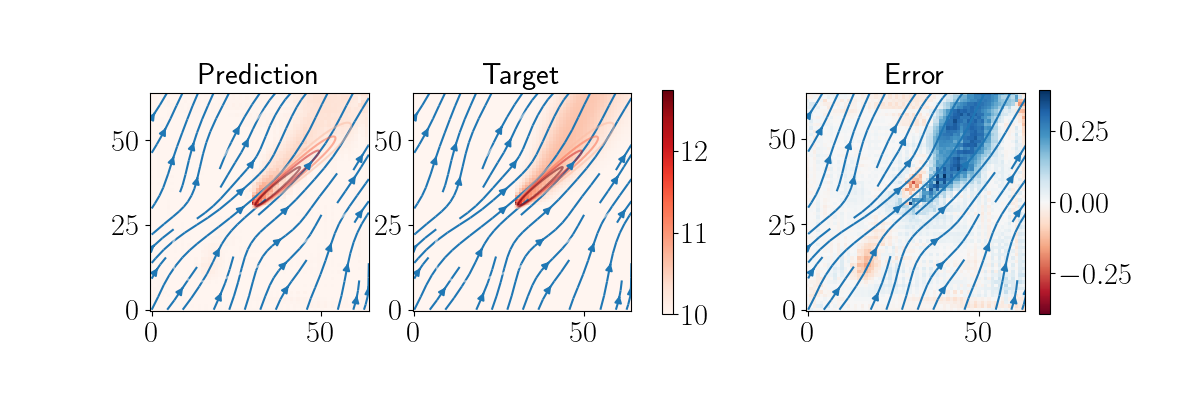
\includegraphics[width=\textwidth]{img/32_comparison_test.png}
      \vspace{-1cm}
   \end{subfigure}
   \begin{subfigure}{0.9\textwidth}
      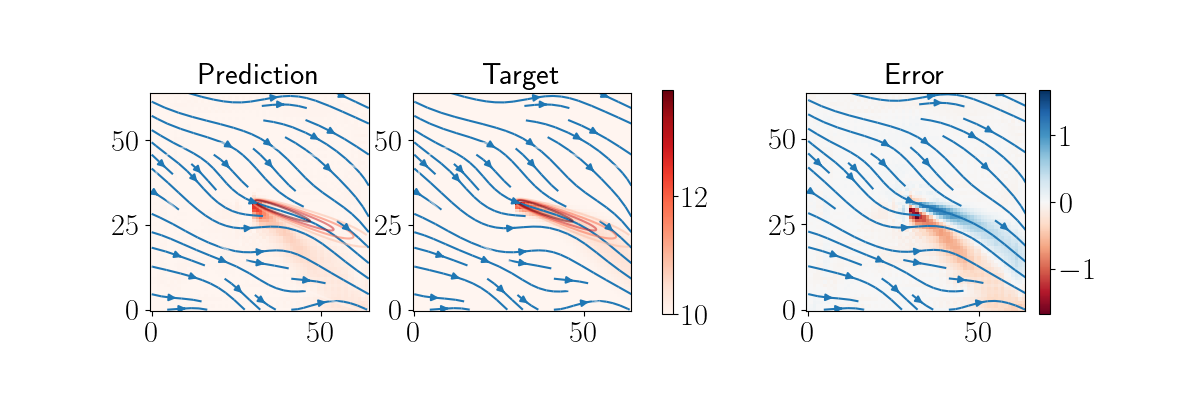
\includegraphics[width=\textwidth]{img/29_comparison_test.png}
      \vspace{-1cm}
   \end{subfigure}
   \caption{Prediction result and simulation ground truth for three different samples from the test data set. The rightmost column displays the error in \degree C. Analytical temperature plumes calculated with the LAHM model are overlaid on top.}
   \label{fig:results}
\end{figure}

% \begin{figure}
%     \centering
%     {\transparent{0.4}\includegraphics[width=0.7\textwidth]{plume.png}}
%     \caption{Caption}
%     \label{fig:my_label}
% \end{figure}

We trained the aforementioned model on a data set of $239$ generated samples. An additional $720$ augmented samples are created by randomly rotating the input and output images resulting in a total data set size of $959$. $192$ of these are randomly selected as validation data during training.
The model is trained using the ADAM optimizer \citep{adam} with a fixed learning rate $0.0004$ for $60000$ epochs.
For further details see Appendix \ref{ap:training_details}.
Fig.~\ref{fig:results} shows a selection of three different predictions of the trained model which were performed using a held out test set of size $40$ which was never before seen by the model.
% These are manually selected from a 
Shown in each row are the model's prediction, the target temperature field from the numerical solution and the point-wise error between the two.
Furthermore the analytical LAHM model from \citet{Pophillat2020} is overlaid on top of both prediction and target plots.
We can nicely observe that in all cases the predicted temperature plume matches the target in direction and shape.
The top example prominently displays the advantage of our method when compared to the analytical model.
While the analytical plume only estimates linear transport of the flow, our method provides a much more detailed prediction following the flow.
The second row again is a nice example of the prediction matching the target quite well also in magnitude.
Lastly, we also include an example where the model did not perform too well and deviates from the expected flow direction showing the predictions are not fully robust yet.
Quantifying the error we see each example having different magnitudes ranging from $0.25$ \degree C to $2$ \degree C.
Note however, that the largest error is often only encountered at the injection site with the rest of the plume showing significantly less errors.
The relative error
\begin{equation*}
    \frac{\sum_i \left| T^p_i - T^t_i \right|}{\sum_i \left| T^t_i \right|}
\end{equation*}
between the predicted temperatures $T^p$ and target temperatures $T^t$ achieved on the complete test data set is $0.68 \%$.
\todo[disable]{this is not so bad, rel. error over whole data set 1\% and high errors mostly due to "small" misalignment of plume}
% All in all these results demonstrate the strengths that our new method provides.
Considering spatial discrepancies of $>10m$ between the analytical model and the higher-fidelity plume predicted by our model, this could make the difference in a real-world scenario when deciding whether it is feasible to place a GWHP on a specific building or not.
\todo[disable]{- evaluation (error on test set, inference time)}
\todo[disable]{e.g. in a real-world scenario a bending plume shifting by ~10m could make the difference when deciding where to place gwhps}
\todo[disable]{- overlay of local surrogates on city map (?)}



% \begin{figure}[htb]
%    \centering
%    \includegraphics[width=10cm,height=6cm]{example-image-a}
%    \caption{Example screenshot of a web app showing multiple hand placed heat pumps on a city map with heat plumes being generated using the surrogate model.}
% \end{figure}


\section{Conclusion}
\label{sec:conclusion}

\todo[disable]{conclusion here, demonstrate feasibility of the method, confident that more compute/examples will further improve in the future}
\todo[disable]{mention inference time? with only ~0.1s this allows real-time applications}
\todo[disable]{- future work: overlapping local predictions $\rightarrow$ resolve with global city-wide model}
In this work we have demonstrated the viability of data-driven surrogate models for approximating subsurface thermal plumes generated by groundwater heat pumps.
With a simple supervised learning approach and a CNN architecture we were able to get a good agreement between fast surrogate predictions and high-fidelity ground truth data.
Especially compared to simpler analytical approaches the data-driven model has shown good results.
This study can be seen as a first step enabling more refined approaches and applications down the line.


Considering the low inference time of the trained model ($\leq 50ms$) we could imagine it being used in close-to-real-time applications such as design tools for city planners.
We would also like to expand the surrogate model by including parametric inputs such as a heat pump's energy output.
Furthermore, a shortcoming of the current approach is the limitation to a small constraint domain with only a single heat pump.
% Even though in this application that scenario is not desirable, other applications might need such interaction.
To model larger scenarios with multiple heat pumps another extension could be stitching together multiple local surrogate predictions and then using these as a preconditioned starting point for solving larger numerical models on the scale of a whole city domain.

\todo[disable]{Web app currently uses analytical model. Want to add this as it uses non-uniform velocities.}

% \section{Submission of conference papers to ICLR 2022}

ICLR requires electronic submissions, processed by
\url{https://openreview.net/}. See ICLR's website for more instructions.

If your paper is ultimately accepted, the statement {\tt
      {\textbackslash}iclrfinalcopy} should be inserted to adjust the
format to the camera ready requirements.

The format for the submissions is a variant of the NeurIPS format.
Please read carefully the instructions below, and follow them
faithfully.

\subsection{Style}

Papers to be submitted to ICLR 2022 must be prepared according to the
instructions presented here.

%% Please note that we have introduced automatic line number generation
%% into the style file for \LaTeXe. This is to help reviewers
%% refer to specific lines of the paper when they make their comments. Please do
%% NOT refer to these line numbers in your paper as they will be removed from the
%% style file for the final version of accepted papers.

Authors are required to use the ICLR \LaTeX{} style files obtainable at the
ICLR website. Please make sure you use the current files and
not previous versions. Tweaking the style files may be grounds for rejection.

\subsection{Retrieval of style files}

The style files for ICLR and other conference information are available online at:
\begin{center}
   \url{http://www.iclr.cc/}
\end{center}
The file \verb+iclr2022_conference.pdf+ contains these
instructions and illustrates the
various formatting requirements your ICLR paper must satisfy.
Submissions must be made using \LaTeX{} and the style files
\verb+iclr2022_conference.sty+ and \verb+iclr2022_conference.bst+ (to be used with \LaTeX{}2e). The file
\verb+iclr2022_conference.tex+ may be used as a ``shell'' for writing your paper. All you
have to do is replace the author, title, abstract, and text of the paper with
your own.

The formatting instructions contained in these style files are summarized in
sections \ref{gen_inst}, \ref{headings}, and \ref{others} below.

\section{General formatting instructions}
\label{gen_inst}

The text must be confined within a rectangle 5.5~inches (33~picas) wide and
9~inches (54~picas) long. The left margin is 1.5~inch (9~picas).
Use 10~point type with a vertical spacing of 11~points. Times New Roman is the
preferred typeface throughout. Paragraphs are separated by 1/2~line space,
with no indentation.

Paper title is 17~point, in small caps and left-aligned.
All pages should start at 1~inch (6~picas) from the top of the page.

Authors' names are
set in boldface, and each name is placed above its corresponding
address. The lead author's name is to be listed first, and
the co-authors' names are set to follow. Authors sharing the
same address can be on the same line.

Please pay special attention to the instructions in section \ref{others}
regarding figures, tables, acknowledgments, and references.


There will be a strict upper limit of 9 pages for the main text of the initial submission, with unlimited additional pages for citations.

\section{Headings: first level}
\label{headings}

First level headings are in small caps,
flush left and in point size 12. One line space before the first level
heading and 1/2~line space after the first level heading.

\subsection{Headings: second level}

Second level headings are in small caps,
flush left and in point size 10. One line space before the second level
heading and 1/2~line space after the second level heading.

\subsubsection{Headings: third level}

Third level headings are in small caps,
flush left and in point size 10. One line space before the third level
heading and 1/2~line space after the third level heading.

\section{Citations, figures, tables, references}
\label{others}

These instructions apply to everyone, regardless of the formatter being used.

\subsection{Citations within the text}

Citations within the text should be based on the \texttt{natbib} package
and include the authors' last names and year (with the ``et~al.'' construct
for more than two authors). When the authors or the publication are
included in the sentence, the citation should not be in parenthesis using \verb|\citet{}| (as
in ``See \citet{nn_pde1} for more information.''). Otherwise, the citation
should be in parenthesis using \verb|\citep{}| (as in ``Deep learning shows promise to make progress
towards AI~\citep{nn_pde2}.'').

The corresponding references are to be listed in alphabetical order of
authors, in the \textsc{References} section. As to the format of the
references themselves, any style is acceptable as long as it is used
consistently.

\subsection{Footnotes}

Indicate footnotes with a number\footnote{Sample of the first footnote} in the
text. Place the footnotes at the bottom of the page on which they appear.
Precede the footnote with a horizontal rule of 2~inches
(12~picas).\footnote{Sample of the second footnote}

\subsection{Figures}

All artwork must be neat, clean, and legible. Lines should be dark
enough for purposes of reproduction; art work should not be
hand-drawn. The figure number and caption always appear after the
figure. Place one line space before the figure caption, and one line
space after the figure. The figure caption is lower case (except for
first word and proper nouns); figures are numbered consecutively.

Make sure the figure caption does not get separated from the figure.
Leave sufficient space to avoid splitting the figure and figure caption.

You may use color figures.
However, it is best for the
figure captions and the paper body to make sense if the paper is printed
either in black/white or in color.
\begin{figure}[h]
   \begin{center}
      %\framebox[4.0in]{$\;$}
      \fbox{\rule[-.5cm]{0cm}{4cm} \rule[-.5cm]{4cm}{0cm}}
   \end{center}
   \caption{Sample figure caption.}
\end{figure}

\subsection{Tables}

All tables must be centered, neat, clean and legible. Do not use hand-drawn
tables. The table number and title always appear before the table. See
Table~\ref{sample-table}.

Place one line space before the table title, one line space after the table
title, and one line space after the table. The table title must be lower case
(except for first word and proper nouns); tables are numbered consecutively.

\begin{table}[t]
   \caption{Sample table title}
   \label{sample-table}
   \begin{center}
      \begin{tabular}{ll}
         \multicolumn{1}{c}{\bf PART} & \multicolumn{1}{c}{\bf DESCRIPTION}
         \\ \hline \\
         Dendrite                     & Input terminal                      \\
         Axon                         & Output terminal                     \\
         Soma                         & Cell body (contains cell nucleus)   \\
      \end{tabular}
   \end{center}
\end{table}

\section{Default Notation}

In an attempt to encourage standardized notation, we have included the
notation file from the textbook, \textit{Deep Learning}
\cite{goodfellow2016deep} available at
\url{https://github.com/goodfeli/dlbook_notation/}.  Use of this style
is not required and can be disabled by commenting out
\texttt{math\_commands.tex}.


\centerline{\bf Numbers and Arrays}
\bgroup
\def\arraystretch{1.5}
\begin{tabular}{p{1in}p{3.25in}}
   $\displaystyle a$                & A scalar (integer or real)                                               \\
   $\displaystyle \va$              & A vector                                                                 \\
   $\displaystyle \mA$              & A matrix                                                                 \\
   $\displaystyle \tA$              & A tensor                                                                 \\
   $\displaystyle \mI_n$            & Identity matrix with $n$ rows and $n$ columns                            \\
   $\displaystyle \mI$              & Identity matrix with dimensionality implied by context                   \\
   $\displaystyle \ve^{(i)}$        & Standard basis vector $[0,\dots,0,1,0,\dots,0]$ with a 1 at position $i$ \\
   $\displaystyle \text{diag}(\va)$ & A square, diagonal matrix with diagonal entries given by $\va$           \\
   $\displaystyle \ra$              & A scalar random variable                                                 \\
   $\displaystyle \rva$             & A vector-valued random variable                                          \\
   $\displaystyle \rmA$             & A matrix-valued random variable                                          \\
\end{tabular}
\egroup
\vspace{0.25cm}

\centerline{\bf Sets and Graphs}
\bgroup
\def\arraystretch{1.5}

\begin{tabular}{p{1.25in}p{3.25in}}
   $\displaystyle \sA$                   & A set                                                                                 \\
   $\displaystyle \R$                    & The set of real numbers                                                               \\
   $\displaystyle \{0, 1\}$              & The set containing 0 and 1                                                            \\
   $\displaystyle \{0, 1, \dots, n \}$   & The set of all integers between $0$ and $n$                                           \\
   $\displaystyle [a, b]$                & The real interval including $a$ and $b$                                               \\
   $\displaystyle (a, b]$                & The real interval excluding $a$ but including $b$                                     \\
   $\displaystyle \sA \backslash \sB$    & Set subtraction, i.e., the set containing the elements of $\sA$ that are not in $\sB$ \\
   $\displaystyle \gG$                   & A graph                                                                               \\
   $\displaystyle \parents_\gG(\ervx_i)$ & The parents of $\ervx_i$ in $\gG$
\end{tabular}
\vspace{0.25cm}


\centerline{\bf Indexing}
\bgroup
\def\arraystretch{1.5}

\begin{tabular}{p{1.25in}p{3.25in}}
   $\displaystyle \eva_i$         & Element $i$ of vector $\va$, with indexing starting at 1 \\
   $\displaystyle \eva_{-i}$      & All elements of vector $\va$ except for element $i$      \\
   $\displaystyle \emA_{i,j}$     & Element $i, j$ of matrix $\mA$                           \\
   $\displaystyle \mA_{i, :}$     & Row $i$ of matrix $\mA$                                  \\
   $\displaystyle \mA_{:, i}$     & Column $i$ of matrix $\mA$                               \\
   $\displaystyle \etA_{i, j, k}$ & Element $(i, j, k)$ of a 3-D tensor $\tA$                \\
   $\displaystyle \tA_{:, :, i}$  & 2-D slice of a 3-D tensor                                \\
   $\displaystyle \erva_i$        & Element $i$ of the random vector $\rva$                  \\
\end{tabular}
\egroup
\vspace{0.25cm}


\centerline{\bf Calculus}
\bgroup
\def\arraystretch{1.5}
\begin{tabular}{p{1.25in}p{3.25in}}
   % NOTE: the [2ex] on the next line adds extra height to that row of the table.
   % Without that command, the fraction on the first line is too tall and collides
   % with the fraction on the second line.
   $\displaystyle\frac{d y} {d x}$                            & Derivative of $y$ with respect to $x$                                  \\ [2ex]
   $\displaystyle \frac{\partial y} {\partial x} $            & Partial derivative of $y$ with respect to $x$                          \\
   $\displaystyle \nabla_\vx y $                              & Gradient of $y$ with respect to $\vx$                                  \\
   $\displaystyle \nabla_\mX y $                              & Matrix derivatives of $y$ with respect to $\mX$                        \\
   $\displaystyle \nabla_\tX y $                              & Tensor containing derivatives of $y$ with respect to $\tX$             \\
   $\displaystyle \frac{\partial f}{\partial \vx} $           & Jacobian matrix $\mJ \in \R^{m\times n}$ of $f: \R^n \rightarrow \R^m$ \\
   $\displaystyle \nabla_\vx^2 f(\vx)\text{ or }\mH( f)(\vx)$ & The Hessian matrix of $f$ at input point $\vx$                         \\
   $\displaystyle \int f(\vx) d\vx $                          & Definite integral over the entire domain of $\vx$                      \\
   $\displaystyle \int_\sS f(\vx) d\vx$                       & Definite integral with respect to $\vx$ over the set $\sS$             \\
\end{tabular}
\egroup
\vspace{0.25cm}

\centerline{\bf Probability and Information Theory}
\bgroup
\def\arraystretch{1.5}
\begin{tabular}{p{1.25in}p{3.25in}}
   $\displaystyle P(\ra)$                                      & A probability distribution over a discrete variable            \\
   $\displaystyle p(\ra)$                                      & A probability distribution over a continuous variable, or over
   a variable whose type has not been specified                                                                                 \\
   $\displaystyle \ra \sim P$                                  & Random variable $\ra$ has distribution $P$                     \\% so thing on left of \sim should always be a random variable, with name beginning with \r
   $\displaystyle  \E_{\rx\sim P} [ f(x) ]\text{ or } \E f(x)$ & Expectation of $f(x)$ with respect to $P(\rx)$                 \\
   $\displaystyle \Var(f(x)) $                                 & Variance of $f(x)$ under $P(\rx)$                              \\
   $\displaystyle \Cov(f(x),g(x)) $                            & Covariance of $f(x)$ and $g(x)$ under $P(\rx)$                 \\
   $\displaystyle H(\rx) $                                     & Shannon entropy of the random variable $\rx$                   \\
   $\displaystyle \KL ( P \Vert Q ) $                          & Kullback-Leibler divergence of P and Q                         \\
   $\displaystyle \mathcal{N} ( \vx ; \vmu , \mSigma)$         & Gaussian distribution                                          %
   over $\vx$ with mean $\vmu$ and covariance $\mSigma$                                                                         \\
\end{tabular}
\egroup
\vspace{0.25cm}

\centerline{\bf Functions}
\bgroup
\def\arraystretch{1.5}
\begin{tabular}{p{1.25in}p{3.25in}}
   $\displaystyle f: \sA \rightarrow \sB$ & The function $f$ with domain $\sA$ and range $\sB$        \\
   $\displaystyle f \circ g $             & Composition of the functions $f$ and $g$                  \\
   $\displaystyle f(\vx ; \vtheta) $      & A function of $\vx$ parametrized by $\vtheta$.
   (Sometimes we write $f(\vx)$ and omit the argument $\vtheta$ to lighten notation)                  \\
   $\displaystyle \log x$                 & Natural logarithm of $x$                                  \\
   $\displaystyle \sigma(x)$              & Logistic sigmoid, $\displaystyle \frac{1} {1 + \exp(-x)}$ \\
   $\displaystyle \zeta(x)$               & Softplus, $\log(1 + \exp(x))$                             \\
   $\displaystyle || \vx ||_p $           & $\normlp$ norm of $\vx$                                   \\
   $\displaystyle || \vx || $             & $\normltwo$ norm of $\vx$                                 \\
   $\displaystyle x^+$                    & Positive part of $x$, i.e., $\max(0,x)$                   \\
   $\displaystyle \1_\mathrm{condition}$  & is 1 if the condition is true, 0 otherwise                \\
\end{tabular}
\egroup
\vspace{0.25cm}



\section{Final instructions}
Do not change any aspects of the formatting parameters in the style files.
In particular, do not modify the width or length of the rectangle the text
should fit into, and do not change font sizes (except perhaps in the
\textsc{References} section; see below). Please note that pages should be
numbered.

\section{Preparing PostScript or PDF files}

Please prepare PostScript or PDF files with paper size ``US Letter'', and
not, for example, ``A4''. The -t
letter option on dvips will produce US Letter files.

Consider directly generating PDF files using \verb+pdflatex+
(especially if you are a MiKTeX user).
PDF figures must be substituted for EPS figures, however.

Otherwise, please generate your PostScript and PDF files with the following commands:
\begin{verbatim}
dvips mypaper.dvi -t letter -Ppdf -G0 -o mypaper.ps
ps2pdf mypaper.ps mypaper.pdf
\end{verbatim}

\subsection{Margins in LaTeX}

Most of the margin problems come from figures positioned by hand using
\verb+\special+ or other commands. We suggest using the command
\verb+\includegraphics+
from the graphicx package. Always specify the figure width as a multiple of
the line width as in the example below using .eps graphics
\begin{verbatim}
   \usepackage[dvips]{graphicx} ...
   \includegraphics[width=0.8\linewidth]{myfile.eps}
\end{verbatim}
or % Apr 2009 addition
\begin{verbatim}
   \usepackage[pdftex]{graphicx} ...
   \includegraphics[width=0.8\linewidth]{myfile.pdf}
\end{verbatim}
for .pdf graphics.
See section~4.4 in the graphics bundle documentation (\url{http://www.ctan.org/tex-archive/macros/latex/required/graphics/grfguide.ps})

A number of width problems arise when LaTeX cannot properly hyphenate a
line. Please give LaTeX hyphenation hints using the \verb+\-+ command.

\subsubsection*{Author Contributions}
If you'd like to, you may include  a section for author contributions as is done
in many journals. This is optional and at the discretion of the authors.

\subsubsection*{Acknowledgments}
Use unnumbered third level headings for the acknowledgments. All
acknowledgments, including those to funding agencies, go at the end of the paper.


\bibliography{iclr2022_conference}
\bibliographystyle{iclr2022_conference}

\appendix
% \section{Appendix}
% You may include other additional sections here.

\section{Training Details}
\label{ap:training_details}
The model was implemented and trained using \emph{PyTorch} \citep{pytorch} on a workstation with two NVIDIA RTX 3090 GPUs. The batch size was fixed at $64$ samples and the ADAM optimizer was used with a learning rate of $4e-4$ and otherwise default parameters.
For supervision a simple MSE loss function is employed.
The model used to produce the results in Sec.~\ref{sec:results} features a total of $480$k parameters.
% The code is available at...
\todo[disable]{add anonymous github repository}

% \begin{figure}[htb]
%   \centering
%   \includegraphics[width=10cm,height=6cm]{example-image-a}
%   \caption{Training progress of the model. Displayed are the total $L_2$ loss and relative error over $n=6000$ epochs.}
% \end{figure}

\section{Simulation Details}
\label{ap:sim_details}
The PFLOTRAN \citep{pflotran-paper} package is used to solve a steady-state thermal-hydrological problem with equations for mass and energy balance given by
\begin{equation}
   \label{eq:mass}
   \nabla \cdot \left(\eta \vq \right) =  \nabla \cdot \left(\eta  K \nabla P  \right) = Q_w
\end{equation}
and
\begin{equation}
   \label{eq:energy}
   \nabla \cdot \left(\eta \vq H\right) - \kappa \Delta T = Q_e
\end{equation}

where $Q_w$ is the mass flow source term, which is non-zero only at the boundaries and at the center where mass is injected into the groundwater by the GWHP, the energy source term $Q_e$, enthalpy $H$, thermal conductivity $\kappa$ and temperature $T$. The relevant parameters are shown in Table \ref{tab:params}.
%with energy source term $Q_e$ in $MW/m^2$ as well as mass source term $Q_w$ in $kmol\, m^{-3} s^{-1}$ and darcy flux $\vq$ in $m/s$

\begin{table}[ht]
\caption{Simulation parameters}
\centering
\begin{tabular}{| c | c | c |}
   \hline
   $\eta$   & molar density        & $55.3454010547$ $kmol/m^3$ \\
   \hline
   $\kappa$ & thermal conductivity & $0.5 W/(mK)$                   \\
   \hline
   H        & specific enthalpy of water at 10\degree C         & $1.134945 kJ/mol$                  \\
   \hline
\end{tabular}
\label{tab:params}
\end{table}

% \section{Physical Constraints}
% \label{ap:phys_constraints}
% Additionally, we use \cref{eq:mass,eq:energy} to regularize the network during training.
% By ensuring that both of these are fulfilled for predictions of the model we steer the training process towards physically plausible solutions which obey mass and energy conservation.
% To achieve this we first calculate the residuals for both equations using sobel filters to get the gradient/divergence fields.
% These residuals are then added to the loss function of the optimizer.

\todo[disable]{- using these we can additionally regularize the network during training}
\todo[disable]{- makes sure that physically plausible solutions are found}
\todo[disable]{- should be more robust?}
\todo[disable]{- comparison with and without physical term (speeds up training?)}


\end{document}
